\documentclass[12pt]{article}
\usepackage{fancyhdr}
\usepackage{amsmath,amsfonts,enumerate,amssymb}
\usepackage{color,graphicx}
\usepackage{float}
\pagestyle{fancy}
\usepackage{soul} %Strikeout
\usepackage{minted}
\usepackage{tikzsymbols}
\usetikzlibrary{arrows}
\newcommand*\circled[1]{\tikz[baseline=(char.base)]{
		\node[shape=circle,draw,inner sep=2pt] (char) {#1};}}
%%%%%%%%%%%%%%%%%%%%%%%%%%%%%%%%%%%%%%%%%%%%%%%%%
% Do your customization here
%%%%%%%%%%%%%%%%%%%%%%%%%%%%%%%%%%%%%%%%%%%%%%%%%
\newcommand{\masunitnumber}{MH1402}
\newcommand{\examdate}{MAY 2018}
\newcommand{\academicyear}{2017-2018}
\newcommand{\semester}{II}
\newcommand{\coursename}{Algorithms \& Computing II}
\newcommand{\numberofhours}{2}

\newcommand{\ZZ}{\mathbb{Z}}
\newcommand{\CC}{\mathbb{C}}
\newcommand{\RR}{\mathbb{R}}
\newcommand{\FF}{\mathbb{F}}
\newcommand{\EOQ}{\hfill $\square$}
%\DeclareMathOperator{\diam}{diam}
%%%%%%%%%%%%%%%%%%%%%%%%%%%%%%%%%%%%%%%%%%%%%%%%%
% Don't touch anything from here till instructions
% to candidates
%%%%%%%%%%%%%%%%%%%%%%%%%%%%%%%%%%%%%%%%%%%%%%%%%
\lhead{}
\rhead{}
\chead{{\bf NANYANG TECHNOLOGICAL UNIVERSITY}}
\lfoot{}
\rfoot{}
\cfoot{}
\begin{document}
\setlength{\headsep}{5truemm}
\setlength{\headheight}{14.5truemm}
\setlength{\voffset}{-0.45truein}
\renewcommand{\headrulewidth}{0.0pt}
\begin{center}
SEMESTER \semester\ EXAMINATION \academicyear ~SUGGESTED SOLUTION
\end{center}
\begin{center}
{\bf \masunitnumber\ -- \coursename}
\end{center}
\vspace{20truemm}

\noindent \examdate\hspace{55truemm} TIME ALLOWED: \numberofhours\ HOURS

\vspace{19truemm}
\hrule
\vspace{19truemm}
\noindent\underline{INSTRUCTIONS TO CANDIDATES}
\vspace{8truemm}
%%%%%%%%%%%%%%%%%%%%%%%%%%%%%%%%%%%%%%%%%%%%%%%%%%%%%%
% Adjust your instructions here
%%%%%%%%%%%%%%%%%%%%%%%%%%%%%%%%%%%%%%%%%%%%%%%%%%%%%%
\begin{enumerate}
\item This examination paper contains {\bf SEVEN (7)} questions and comprises 
{\bf FOUR (4)} printed pages.

\item Answer all questions. 
The marks for each question are indicated at the beginning of each question.


\item Answer each question beginning on a {\bf FRESH} page of the answer book.

\item This {\bf IS NOT} an {\bf OPEN BOOK} exam.

\item Candidates may use calculators. However, they should write down systematically the steps in the workings.
\end{enumerate}

%%%%%%%%%%%%%%%%%%%%%%%%%%%%%%%%%%%%%%%%%%%%%%%%%
% leave this as it is
%%%%%%%%%%%%%%%%%%%%%%%%%%%%%%%%%%%%%%%%%%%%%%%%%
\newpage
\lhead{}
\rhead{\masunitnumber}
\chead{}
\lfoot{}
\cfoot{\thepage}
\rfoot{}
\setlength{\footskip}{45pt}
%%%%%%%%%%%%%%%%%%%%%%%%%%%%%%%%%%%%%%%%%%%%%%%%%%
% put your exam questions here
%%%%%%%%%%%%%%%%%%%%%%%%%%%%%%%%%%%%%%%%%%%%%%%%%%
\noindent Solutions provided by:
Brandon Goh -- bgoh008@e.ntu.edu.sg
\paragraph{Question 1.}
\begin{enumerate}[(a)]
    \item Show by mathematical induction that $T(n)=2^{n+1}-1$, given the following definition:\hfill{\bf (6 marks)}\\
    \begin{align*}
    T(n)=\left\{
                    \begin{array}{ll}
                      1&\quad \text{if }n=0,\\
                      T(n-1)+2^n&\quad\text{otherwise.}
                    \end{array}
                  \right.
    \end{align*}
    \item What is the complexity of the following piece of Python code in Big-Oh notation? \hfill {\bf 5 marks}
    \begin{minted}[frame=single, framesep=5pt]{python}
sum = 0
for i in range(n**2):
    for j in range(i):
        sum += j
    \end{minted}
\end{enumerate}

\paragraph{Answer}
\begin{enumerate}[(a)]
\item Take the LHS as the given equation and RHS as $T(n)=2^{n+1}-1$.\\\\{\bf Base Case}~~~~$n=0$\\\\(LHS) $T(0)=1$\\(RHS) $T(0)=2^1-1=1$\\\\LHS=RHS, $\therefore$ Base case is true.\\\\{\bf Hypothesis}~~~~$n=k$\\\\Assume that $n=k$ is true, then\\
\begin{equation*}
T(k)=T(k-1)+2^k=2^{k+1}-1
\end{equation*}\\
{\bf Induction}~~~~$n=k+1$\\\\To prove that $n=k+1$ is true, LHS must be equal to RHS.\\\\(RHS) $T(k+1)=2^{k+2}-1$\\(LHS) $T(k+1)=T(k)+2^k\\\vspace{0.04cm}
\text{\hspace{2.83cm}}=(2^{k+1}-1)+2^{k+1}\\\vspace{0.04cm}
\text{\hspace{2.83cm}}=2\cdot 2^{k+1}-1\\\vspace{0.04cm}
\text{\hspace{2.83cm}}=2^{k+2}-1\\\vspace{0.04cm}
\text{\hspace{2.83cm}}=\text{(RHS)}$\\\\From the above, $n=0$ and $n=k$ are true \\$\Rightarrow$ $n=k+1$ is also true. Then by mathematical induction, the equation is true for all $n\in\mathbb{N}_0$.
\EOQ
\item Break the question into 2 blocks:\\\\
Block 1:\\
\verb|sum = 0| $\rightarrow$ 1 operation.\\\\Block 2:\\
\verb|for i in range(n**2):|\\\hspace*{0.6cm}\verb|for j in range(i):|\\\hspace*{1.2cm}\verb|sum += j|\\\\It is important to note that \verb|sum += j| constitutes as 1 operation per execution.\\\\Start by considering small cases.
\begin{enumerate}[(1)]
\item When $n=0$, there is no execution of the \textbf{outer} loop.
\item When $n=1$, $i=0$ only $\Rightarrow$ there is no execution of \textbf{inner} loop.
\item When $n=2$, $i\in\{0,1,2,3\}$
\begin{itemize}
\item \verb|j in range(0)| $\Rightarrow$ inner loop is not executed.
\item \verb|j in range(1)| $\Rightarrow$ inner loop is executed \textbf{once}.
\item \verb|j in range(2)| $\Rightarrow$ inner loop is executed \textbf{twice}.
\item \verb|j in range(3)| $\Rightarrow$ inner loop is executed \textbf{thrice}.
\end{itemize}
Total executions: $\sum\limits_{x=1}^{3}x=6$
\end{enumerate}
\item When $n=3$, $i\in\{0,1,2,3,4,5,6,7,8\}$
\begin{itemize}
\item \verb|j in range(0)| $\Rightarrow$ inner loop is not executed.
\item \verb|j in range(1)| $\Rightarrow$ inner loop is executed \textbf{once}.
\item \verb|j in range(2)| $\Rightarrow$ inner loop is executed \textbf{twice}.
\item {$\vdots$}
\item \verb|j in range(8)| $\Rightarrow$ inner loop is executed \textbf{eight} times.
\end{itemize}
Total executions: $\sum\limits_{x=1}^{8}x=36$
\end{enumerate}
Using the inner loops, we determine that the number of executions can be simplified to the following:
\begin{equation*}
\sum_{x=1}^{\max(i)}x
\end{equation*}
Now consider the outer loop, the number of executions of the inner loop is based on the value of $n$. Furthermore, $i$ depends on $n$. The formula for the total number of executions can be written in the following form.
\begin{equation*}
\sum_{j=1}^{n}\sum_{x=1}^{j^2-1}x
\end{equation*}
Solving the double summation yields the following the result.
\begin{equation*}
\begin{split}
\sum_{j=1}^{n}\sum_{x=1}^{j^2-1}x&=\sum_{j=1}^{n}\frac{(j^2-1)(j^2)}{2}\\&=\frac{1}{20}(n-1)(n)(n+1)(n+2)(2n+1)\\
&=O(n^5)
\end{split}
\end{equation*}
Note: You are \textbf{NOT} required to know the result from the double summation. Instead, you are expected to know that $\sum\limits_{x=1}^{n}x^a=O(x^{a+1})$ where $a\in\mathbb{N}_0$.\\\\The loop gives us a time complexity of $O(n^5)$, so the addition of the 1 operation from outside the loop ($O(1)$) will not change the time complexity of the algorithm.\EOQ
\paragraph{Question 2.} Given the following binary search tree

\begin{figure}[H]
		\centering
		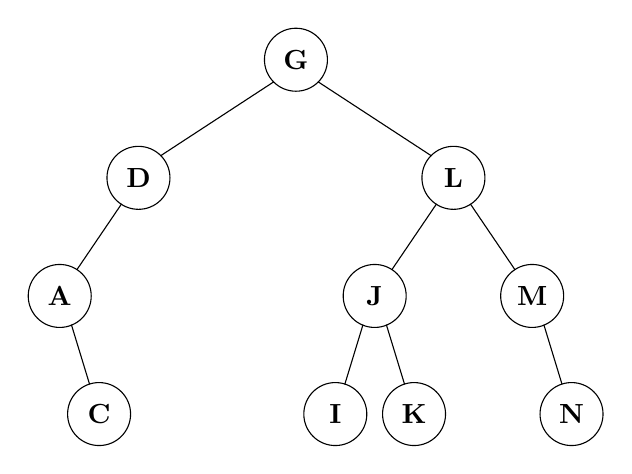
\begin{tikzpicture}	
		%Depth 0
		\draw (0,0) circle (0.4cm) node {\bf G};
		\draw (-0.279,-0.279)--(-1.721,-1.221);
		\draw (0.279,-0.279)--(1.721,-1.221);
		%Depth 1
		\draw (-2,-1.5) circle(0.4cm) node {\bf D};
		\draw (2,-1.5) circle(0.4cm) node {\bf L};
		\draw(-2.214,-1.83)--(-2.784,-2.67);
		\draw(1.786,-1.83)--(1.216,-2.67);
		\draw(2.214,-1.83)--(2.784,-2.67);
		%Depth 2
		\draw (-3,-3) circle(0.4cm) node {\bf A};
		\draw (1,-3) circle(0.4cm) node {\bf J};
		\draw (3,-3) circle(0.4cm) node {\bf M};
		\draw(-2.852,-3.364)--(-2.62,-4.124);
		\draw(1.148,-3.364)--(1.38,-4.124);
		\draw(0.852,-3.364)--(0.62,-4.124);
		\draw(3.148,-3.364)--(3.38,-4.124);
		%Depth 3
		\draw (-2.5,-4.5) circle(0.4cm) node {\bf C};
		\draw (0.5,-4.5) circle(0.4cm) node {\bf I};
		\draw (1.5,-4.5) circle(0.4cm) node {\bf K};
		\draw (3.5,-4.5) circle(0.4cm) node {\bf N};
		
		\end{tikzpicture}
		\caption{Binary Search Tree}
		\label{fig:BST}
	\end{figure}

\begin{enumerate}[(a)]
\item What is the sequence of nodes by Euler's Traversal? \hfill {\bf (8 marks)}
\item Draw the resultant tree after removing node ``L''. \hfill {\bf (6 marks)}
\end{enumerate}
\paragraph{Answer}
\begin{enumerate}[(a)]
\item $G\rightarrow D\rightarrow A\rightarrow C\rightarrow A\rightarrow D\rightarrow G\rightarrow L\rightarrow J\rightarrow I\rightarrow J\rightarrow K\rightarrow J\rightarrow L\rightarrow M\rightarrow N\rightarrow M\rightarrow L\rightarrow G$ \EOQ
\item Step 1: L has 2 child nodes, so the key must be swapped with its \textbf{successor}.
\begin{figure}[H]
		\centering
		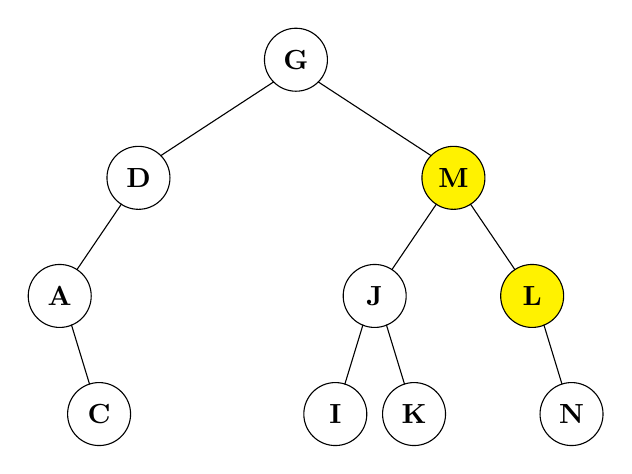
\begin{tikzpicture}	
		%Depth 0
		\draw (0,0) circle (0.4cm) node {\bf G};
		\draw (-0.279,-0.279)--(-1.721,-1.221);
		\draw (0.279,-0.279)--(1.721,-1.221);
		%Depth 1
		\draw (-2,-1.5) circle(0.4cm) node {\bf D};
		\draw[fill=yellow] (2,-1.5) circle(0.4cm) node {\bf M};
		\draw(-2.214,-1.83)--(-2.784,-2.67);
		\draw(1.786,-1.83)--(1.216,-2.67);
		\draw(2.214,-1.83)--(2.784,-2.67);
		%Depth 2
		\draw (-3,-3) circle(0.4cm) node {\bf A};
		\draw (1,-3) circle(0.4cm) node {\bf J};
		\draw[fill=yellow] (3,-3) circle(0.4cm) node {\bf L};
		\draw(-2.852,-3.364)--(-2.62,-4.124);
		\draw(1.148,-3.364)--(1.38,-4.124);
		\draw(0.852,-3.364)--(0.62,-4.124);
		\draw(3.148,-3.364)--(3.38,-4.124);
		%Depth 3
		\draw (-2.5,-4.5) circle(0.4cm) node {\bf C};
		\draw (0.5,-4.5) circle(0.4cm) node {\bf I};
		\draw (1.5,-4.5) circle(0.4cm) node {\bf K};
		\draw (3.5,-4.5) circle(0.4cm) node {\bf N};
		
		\end{tikzpicture}
		\caption{Binary Search Tree After Step 1}
		\label{fig:BSTS1}
	\end{figure}
	Step 2: L now has 1 child node, so swap the key with the child.
	\begin{figure}[H]
			\centering
			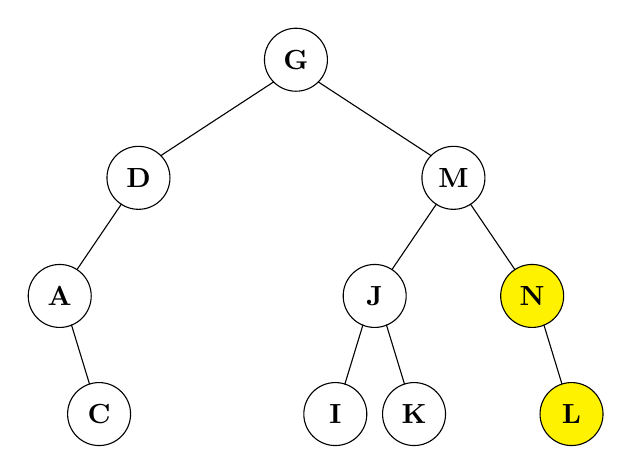
\begin{tikzpicture}	
			%Depth 0
			\draw (0,0) circle (0.4cm) node {\bf G};
			\draw (-0.279,-0.279)--(-1.721,-1.221);
			\draw (0.279,-0.279)--(1.721,-1.221);
			%Depth 1
			\draw (-2,-1.5) circle(0.4cm) node {\bf D};
			\draw (2,-1.5) circle(0.4cm) node {\bf M};
			\draw(-2.214,-1.83)--(-2.784,-2.67);
			\draw(1.786,-1.83)--(1.216,-2.67);
			\draw(2.214,-1.83)--(2.784,-2.67);
			%Depth 2
			\draw (-3,-3) circle(0.4cm) node {\bf A};
			\draw (1,-3) circle(0.4cm) node {\bf J};
			\draw[fill=yellow] (3,-3) circle(0.4cm) node {\bf N};
			\draw(-2.852,-3.364)--(-2.62,-4.124);
			\draw(1.148,-3.364)--(1.38,-4.124);
			\draw(0.852,-3.364)--(0.62,-4.124);
			\draw(3.148,-3.364)--(3.38,-4.124);
			%Depth 3
			\draw (-2.5,-4.5) circle(0.4cm) node {\bf C};
			\draw (0.5,-4.5) circle(0.4cm) node {\bf I};
			\draw (1.5,-4.5) circle(0.4cm) node {\bf K};
			\draw[fill=yellow] (3.5,-4.5) circle(0.4cm) node {\bf L};
			
			\end{tikzpicture}
			\caption{Binary Search Tree After Step 2}
			\label{fig:BSTS2}
		\end{figure}
		Step 3: L has no child nodes, so remove the node from the BST.
		\begin{figure}[H]
					\centering
					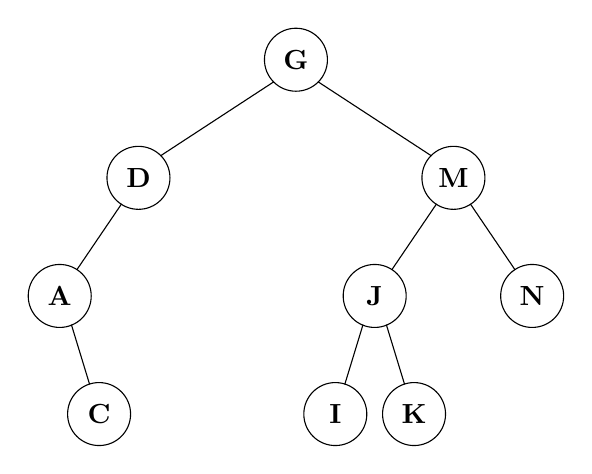
\begin{tikzpicture}	
					%Depth 0
					\draw (0,0) circle (0.4cm) node {\bf G};
					\draw (-0.279,-0.279)--(-1.721,-1.221);
					\draw (0.279,-0.279)--(1.721,-1.221);
					%Depth 1
					\draw (-2,-1.5) circle(0.4cm) node {\bf D};
					\draw (2,-1.5) circle(0.4cm) node {\bf M};
					\draw(-2.214,-1.83)--(-2.784,-2.67);
					\draw(1.786,-1.83)--(1.216,-2.67);
					\draw(2.214,-1.83)--(2.784,-2.67);
					%Depth 2
					\draw (-3,-3) circle(0.4cm) node {\bf A};
					\draw (1,-3) circle(0.4cm) node {\bf J};
					\draw (3,-3) circle(0.4cm) node {\bf N};
					\draw(-2.852,-3.364)--(-2.62,-4.124);
					\draw(1.148,-3.364)--(1.38,-4.124);
					\draw(0.852,-3.364)--(0.62,-4.124);
					%Depth 3
					\draw (-2.5,-4.5) circle(0.4cm) node {\bf C};
					\draw (0.5,-4.5) circle(0.4cm) node {\bf I};
					\draw (1.5,-4.5) circle(0.4cm) node {\bf K};
					
					\end{tikzpicture}
					\caption{Final Binary Search Tree}
					\label{fig:BSTF}
				\end{figure}\EOQ
\end{enumerate}
\newpage
\paragraph{Question 3.} Given the node class implementation below:
\begin{minted}[frame=single, framesep=5pt]{python}
class Node:
    def __init__(self, initElement):
        self.left = None              #left child
        self.right = None             #right child
        self.parent = None            #parent
        self.element = initElement
\end{minted}
write in Python a \textit{function} to print the element of all nodes of a binary tree in the order of depth, i.e., the node of depth 0 first (the root), followed by all the nodes of depth 1 (children of the root), then all the nodes of depth 2 (grandchildren of the root) ..., until all the nodes are printed. The function takes the root node of the binary tree as input. You may assume the Queue class is available for use, including functions like:
\begin{itemize}
\item Queue(): instantiate an empty queue,
\item enqueue(Node x): enqueue node x,
\item dequeue(): dequeue and returns the node removed from queue,
\item isEmpty(): returns \textit{True} if queue is empty, \textit{False} otherwise.
\end{itemize}
Note the input binary tree may or may not be a proper binary tree. \\\text{}\hfill \textbf{(12 marks)}
\paragraph{Answer}\mbox{}\\\\
Since the question only requires us to print the nodes in order without any particular formatting, the code below satisfies the requirements.\\
\begin{minted}{python}
def TreeOrder(root):
    A=Queue()                   #Create empty queue A
    A.enqueue(root)             #Queue the root node
    while not A.isEmpty():      #The queue is not-empty,
                                #so there are nodes that 
                                #still need to be processed
        P=A.dequeue()           #Remove node for processing
        print(P.element)        #Print element in the node
        if P.left!=None:         
            A.enqueue(P.left)   #Queue left child node if exists
        if P.right!=None:        
            A.enqueue(P.right)  #Queue right child node if exists
    return
\end{minted}
\EOQ
\paragraph{Question 4.} Consider the list L $=[1,4,2,8,6,3,5]$.
\begin{enumerate}[(a)]
\item Apply merge-sort algorithm on the list L. Explain with a binary tree the successive recursive calls, and another binary tree the successive merge processes. Assume the left part takes half or one element less, i.e. $\lfloor n/2\rfloor$ when dividing a sub-problem of size $n$. \hfill {\bf (12 marks)}
\item Apply quick-sort algorithm on the original list L. Explain with a binary tree the sort process and underline the pivots. Assume it is always the second element of current sub-problem selected as the pivot.\\\mbox{}\hfill {\bf (12 marks)}
\end{enumerate}
\paragraph{Answer}
\begin{enumerate}[(a)]
\item First Binary Tree for Successive Recursive Calls
\begin{figure}[H]
\centering
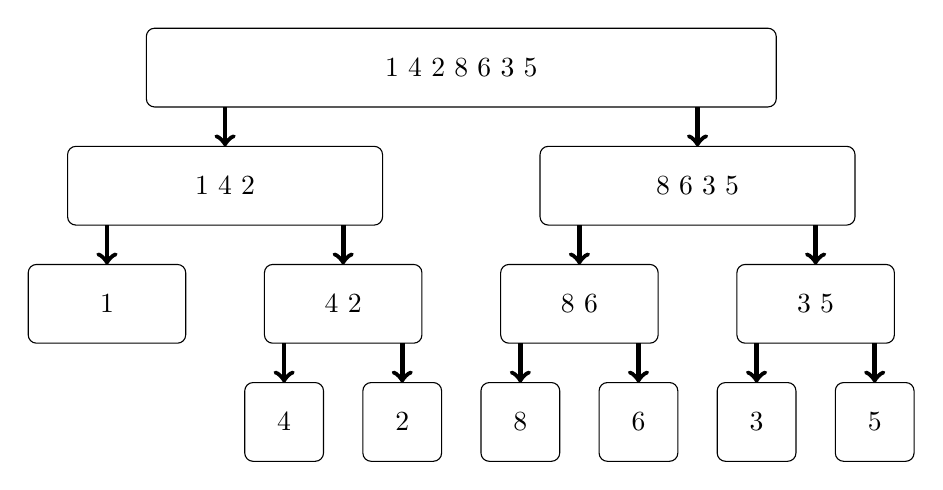
\begin{tikzpicture}	
%Depth 0
\draw[rounded corners=3pt] (-4,0) rectangle node {1   4   2   8   6   3   5} (4,-1) ;


\draw[rounded corners=3pt] (-5,-1.5) rectangle node {1   4   2} (-1,-2.5) ;
\draw[rounded corners=3pt] (1,-1.5) rectangle node {8   6   3   5} (5,-2.5) ;
\draw[<-,line width=0.6mm] (-3,-1.5)--(-3,-1);
\draw[<-,line width=0.6mm] (3,-1.5)--(3,-1);


\draw[rounded corners=3pt] (-5.5,-3) rectangle node {1} (-3.5,-4) ;
\draw[rounded corners=3pt] (-2.5,-3) rectangle node {4   2 } (-0.5,-4) ;
\draw[rounded corners=3pt] (0.5,-3) rectangle node {8   6} (2.5,-4) ;
\draw[rounded corners=3pt] (3.5,-3) rectangle node {3   5} (5.5,-4) ;
\draw[<-, line width=0.6mm] (-4.5,-3)--(-4.5,-2.5);
\draw[<-, line width=0.6mm] (-1.5,-3) -- (-1.5,-2.5);
\draw[<-, line width=0.6mm] (1.5,-3) -- (1.5,-2.5);
\draw[<-, line width=0.6mm] (4.5,-3)--(4.5,-2.5);

\draw[rounded corners=3pt] (-2.75,-4.5) rectangle node {4} (-1.75,-5.5) ;
\draw[rounded corners=3pt] (-0.25,-4.5) rectangle node {2} (-1.25,-5.5) ;
\draw[rounded corners=3pt] (0.25,-4.5) rectangle node {8} (1.25,-5.5) ;
\draw[rounded corners=3pt] (1.75,-4.5) rectangle node {6} (2.75,-5.5) ;
\draw[rounded corners=3pt] (3.25,-4.5) rectangle node {3} (4.25,-5.5) ;
\draw[rounded corners=3pt] (4.75,-4.5) rectangle node {5} (5.75,-5.5) ;
\draw[<-, line width=0.6mm] (-2.25,-4.5)--(-2.25,-4);
\draw[<-, line width=0.6mm] (-0.75,-4.5)--(-0.75,-4);
\draw[<-, line width=0.6mm] (0.75,-4.5)--(0.75,-4);
\draw[<-, line width=0.6mm] (2.25,-4.5)--(2.25,-4);
\draw[<-, line width=0.6mm] (3.75,-4.5)--(3.75,-4);
\draw[<-, line width=0.6mm] (5.25,-4.5)--(5.25,-4);

\end{tikzpicture}
\caption{Binary Tree for Mergesort (Splitting)}
\label{fig:MS1}
\end{figure}
Second Binary Tree for Sorting
\begin{figure}[H]
\centering
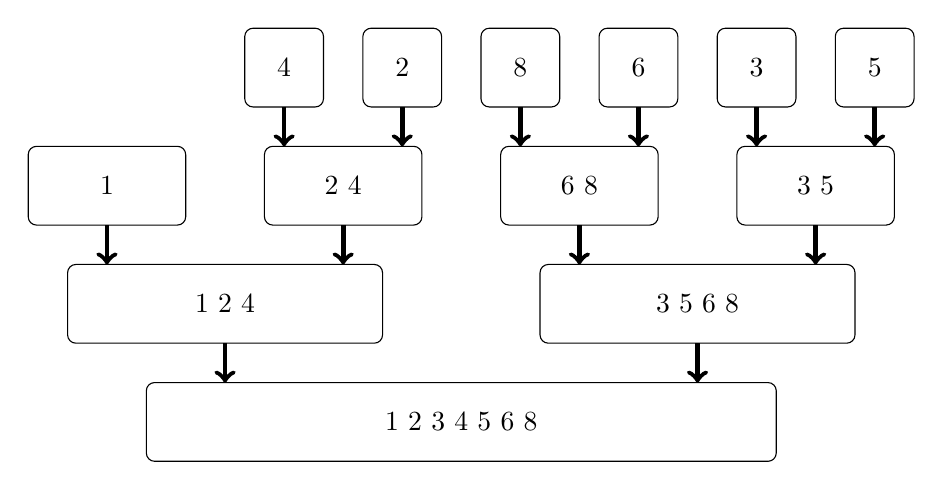
\begin{tikzpicture}	
%Depth 0
\draw[rounded corners=3pt] (-4,0) rectangle node {1   2   3   4   5   6   8} (4,1) ;


\draw[rounded corners=3pt] (-5,1.5) rectangle node {1   2   4} (-1,2.5) ;
\draw[rounded corners=3pt] (1,1.5) rectangle node {3   5   6   8} (5,2.5) ;
\draw[->,line width=0.6mm] (-3,1.5)--(-3,1);
\draw[->,line width=0.6mm] (3,1.5)--(3,1);


\draw[rounded corners=3pt] (-5.5,3) rectangle node {1} (-3.5,4) ;
\draw[rounded corners=3pt] (-2.5,3) rectangle node {2   4} (-0.5,4) ;
\draw[rounded corners=3pt] (0.5,3) rectangle node {6   8} (2.5,4) ;
\draw[rounded corners=3pt] (3.5,3) rectangle node {3   5} (5.5,4) ;
\draw[->, line width=0.6mm] (-4.5,3)--(-4.5,2.5);
\draw[->, line width=0.6mm] (-1.5,3) -- (-1.5,2.5);
\draw[->, line width=0.6mm] (1.5,3) -- (1.5,2.5);
\draw[->, line width=0.6mm] (4.5,3)--(4.5,2.5);

\draw[rounded corners=3pt] (-2.75,4.5) rectangle node {4} (-1.75,5.5) ;
\draw[rounded corners=3pt] (-0.25,4.5) rectangle node {2} (-1.25,5.5) ;
\draw[rounded corners=3pt] (0.25,4.5) rectangle node {8} (1.25,5.5) ;
\draw[rounded corners=3pt] (1.75,4.5) rectangle node {6} (2.75,5.5) ;
\draw[rounded corners=3pt] (3.25,4.5) rectangle node {3} (4.25,5.5) ;
\draw[rounded corners=3pt] (4.75,4.5) rectangle node {5} (5.75,5.5) ;
\draw[->, line width=0.6mm] (-2.25,4.5)--(-2.25,4);
\draw[->, line width=0.6mm] (-0.75,4.5)--(-0.75,4);
\draw[->, line width=0.6mm] (0.75,4.5)--(0.75,4);
\draw[->, line width=0.6mm] (2.25,4.5)--(2.25,4);
\draw[->, line width=0.6mm] (3.75,4.5)--(3.75,4);
\draw[->, line width=0.6mm] (5.25,4.5)--(5.25,4);

\end{tikzpicture}
\caption{Binary Tree for Mergesort (Merging)}
\label{fig:MS2}
\end{figure}
\item Binary Tree for quicksort
\begin{figure}[H]
\centering
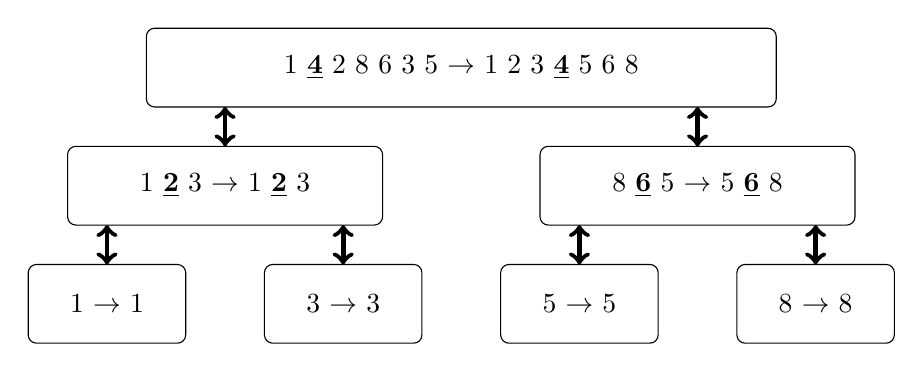
\begin{tikzpicture}	
%Depth 0
\draw[rounded corners=3pt] (-4,0) rectangle node {1   \underline{\textbf{4}}   2   8   6   3   5   $\rightarrow$   1   2   3   \underline{\textbf{4}}   5   6   8} (4,-1) ;

\draw[rounded corners=3pt] (-5,-1.5) rectangle node {1   \underline{\textbf{2}}   3   $\rightarrow$   1   \underline{\textbf{2}}   3} (-1,-2.5) ;
\draw[rounded corners=3pt] (1,-1.5) rectangle node {8   \underline{\textbf{6}}   5   $\rightarrow$   5   \underline{\textbf{6}}   8} (5,-2.5) ;
\draw[<->,line width=0.6mm] (-3,-1.5)--(-3,-1);
\draw[<->,line width=0.6mm] (3,-1.5)--(3,-1);


\draw[rounded corners=3pt] (-5.5,-3) rectangle node {1   $\rightarrow$   1} (-3.5,-4) ;
\draw[rounded corners=3pt] (-2.5,-3) rectangle node {3   $\rightarrow$   3} (-0.5,-4) ;
\draw[rounded corners=3pt] (0.5,-3) rectangle node {5   $\rightarrow$   5} (2.5,-4) ;
\draw[rounded corners=3pt] (3.5,-3) rectangle node {8   $\rightarrow$   8} (5.5,-4) ;
\draw[<->, line width=0.6mm] (-4.5,-3)--(-4.5,-2.5);
\draw[<->, line width=0.6mm] (-1.5,-3) -- (-1.5,-2.5);
\draw[<->, line width=0.6mm] (1.5,-3) -- (1.5,-2.5);
\draw[<->, line width=0.6mm] (4.5,-3)--(4.5,-2.5);
\end{tikzpicture}
\caption{Binary Tree for Quicksort}
\label{fig:QS}
\end{figure}
\noindent
Step \circled{1} \\Identify pivot\\\\
Step \circled{2} \\Split the values into the left and right subtrees respectively depending on whether the values are less than ($<$) or greater than ($>$) the pivot (while preserving the order).\\\\
Step \circled{3} \\Arrays of length 1 are already sorted (trivial).\\\\
Step \circled{4} \\ Combine after obtaining the results from the child nodes. \EOQ
\end{enumerate}
\paragraph{Question 5.} Give the frequency table, Huffman tree, and the resulting table of code words of all characters for the string ``aabaabccdbea''. Note that subtree with more nodes is always placed on the right when joining two subtrees.\hfill {\bf (15 marks)}
\paragraph{Answer}\mbox{}\\\\
Frequency table:
\begin{table}[H]
\centering
\begin{tabular}{|c|c|c|c|c|}
\hline
a & b & c & d & e \\ \hline
5 & 3 & 2 & 1 & 1 \\ \hline
\end{tabular}
\end{table}
\noindent When drawn in its node form:
\begin{figure}[H]
\centering
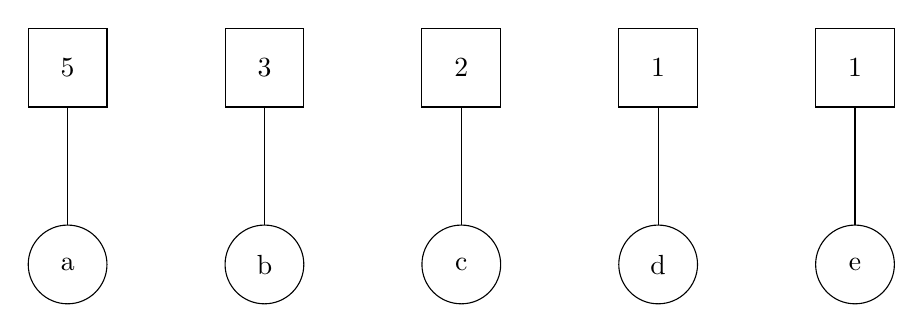
\begin{tikzpicture}[node distance=2.5cm]

\tikzstyle{ci} = [circle,minimum height=1cm, text centered, draw=black]
\tikzstyle{sq} = [rectangle,minimum height=1cm, minimum width=1cm, text centered, draw=black]
\node (afreq) [sq] {5};
\node (a) [ci, below of=afreq] {a};
\node (bfreq) [sq, right of=afreq] {3};
\node (b) [ci, below of=bfreq] {b};
\node (cfreq) [sq, right of =bfreq] {2};
\node (c) [ci, below of=cfreq] {c};
\node (dfreq) [sq, right of =cfreq] {1};
\node (d) [ci, below of=dfreq] {d};
\node (efreq) [sq, right of =dfreq] {1};
\node (e) [ci, below of=efreq] {e}; 
\draw (afreq)--(a);
\draw (bfreq)--(b);
\draw (cfreq)--(c);
\draw (dfreq)--(d);
\draw (efreq)--(e);
\end{tikzpicture}
\end{figure}
\noindent
When computing the Huffman Tree, always combine the nodes of letters (or data) with the two lowest frequencies. In this case, $d$ and $e$ both have the lowest frequency of 1.\\
\begin{figure}[H]
\centering
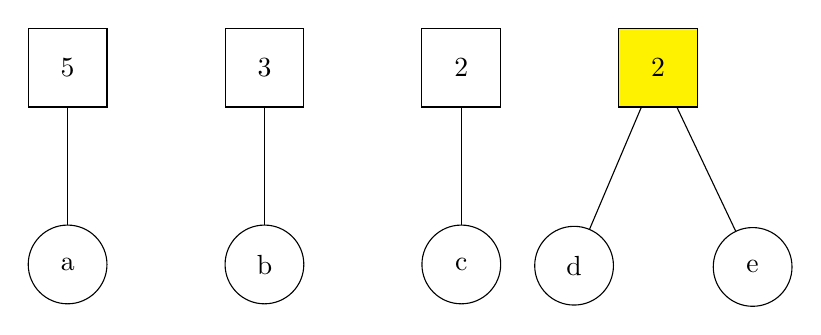
\begin{tikzpicture}[node distance=2.5cm]

\tikzstyle{ci} = [circle,minimum height=1cm, text centered, draw=black]
\tikzstyle{sq} = [rectangle,minimum height=1cm, minimum width=1cm, text centered, draw=black]
\node (afreq) [sq] {5};
\node (a) [ci, below of=afreq] {a};
\node (bfreq) [sq, right of=afreq] {3};
\node (b) [ci, below of=bfreq] {b};
\node (cfreq) [sq, right of =bfreq] {2};
\node (c) [ci, below of=cfreq] {c};
\node (edfreq) [sq, right of=cfreq,fill=yellow] {2};
\node (d) [ci, below left of=edfreq, right of=c,xshift=0.7cm,yshift=1.752cm] {d};
\node (e) [ci, below right of=edfreq, right of=d,xshift=-2cm,yshift=1.752cm] {e}; 
\draw (afreq)--(a);
\draw (bfreq)--(b);
\draw (cfreq)--(c);
\draw (edfreq)--(d);
\draw (edfreq)--(e);
\end{tikzpicture}
\end{figure}
\noindent Now, $c$ \& ($d$ \& $e$) have the lowest frequencies. Therefore, we will combine these two branches.
\begin{figure}[H]
\centering
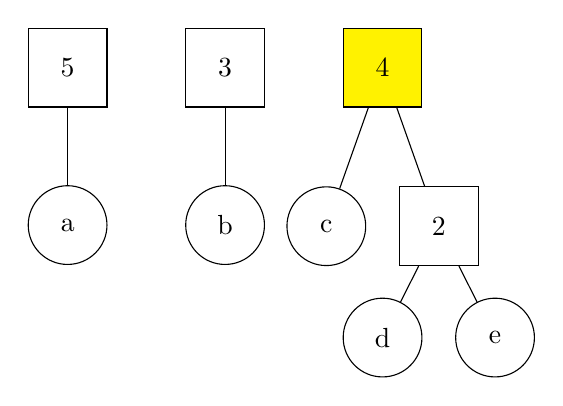
\begin{tikzpicture}[node distance=2cm]

\tikzstyle{ci} = [circle,minimum height=1cm, text centered, draw=black]
\tikzstyle{sq} = [rectangle,minimum height=1cm, minimum width=1cm, text centered, draw=black]
\node (afreq) [sq] {5};
\node (a) [ci, below of=afreq] {a};
\node (bfreq) [sq, right of=afreq] {3};
\node (b) [ci, below of=bfreq] {b};
\node (cfreq) [sq, right of =bfreq,fill=yellow] {4};
\node (c) [ci, below left of=cfreq,xshift=0.7cm,yshift=-0.6cm] {c};
\node (edfreq) [sq, below right of=cfreq,xshift=-0.7cm, yshift=-0.6cm] {2};
\node (d) [ci, below left of=edfreq,xshift=0.7cm] {d};
\node (e) [ci, below right of=edfreq,xshift=-0.7cm] {e}; 
\draw (afreq)--(a);
\draw (bfreq)--(b);
\draw (cfreq)--(c);
\draw (edfreq)--(d);
\draw (edfreq)--(e);
\draw (edfreq)--(cfreq);
\end{tikzpicture}
\end{figure}
\noindent Again, $b$ \& ($c$ \& ($d$ \& $e$)) have the lowest frequencies. Note that b has 3 nodes while ($c$ \& ($d$ \& $e$)) has 4 nodes. As such, b is on the left subtree.

\begin{figure}[H]
\centering
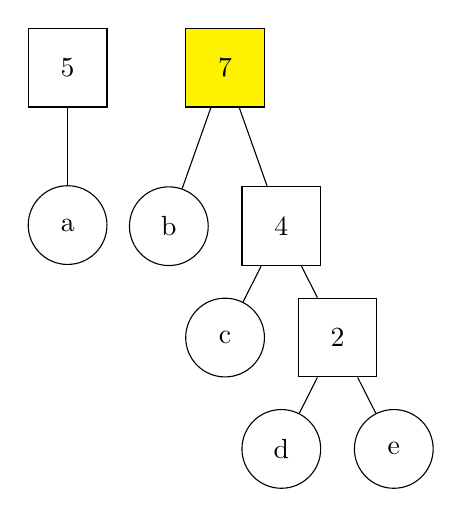
\begin{tikzpicture}[node distance=2cm]

\tikzstyle{ci} = [circle,minimum height=1cm, text centered, draw=black]
\tikzstyle{sq} = [rectangle,minimum height=1cm, minimum width=1cm, text centered, draw=black]
\node (afreq) [sq] {5};
\node (a) [ci, below of=afreq] {a};
\node (bfreq) [sq, right of=afreq,fill=yellow] {7};
\node (b) [ci, below left of=bfreq,yshift=-0.6cm,xshift=0.7cm] {b};
\node (cfreq) [sq, below right of =bfreq,yshift=-0.6cm,xshift=-0.7cm] {4};
\node (c) [ci, below left of=cfreq,xshift=0.7cm] {c};
\node (edfreq) [sq, below right of=cfreq,xshift=-0.7cm] {2};
\node (d) [ci, below left of=edfreq,xshift=0.7cm] {d};
\node (e) [ci, below right of=edfreq,xshift=-0.7cm] {e}; 
\draw (afreq)--(a);
\draw (bfreq)--(b);
\draw (cfreq)--(c);
\draw (edfreq)--(d);
\draw (edfreq)--(e);
\draw (edfreq)--(cfreq);
\draw (bfreq) -- (cfreq);
\end{tikzpicture}
\end{figure}
\noindent
Finally, $a$ \& ($b$ \& ($c$ \& ($d$ \& $e$))) are the last two roots of their respective subtrees. Both subtrees can be merged together, with $a$ on the left subtree.

\begin{figure}[H]
\centering
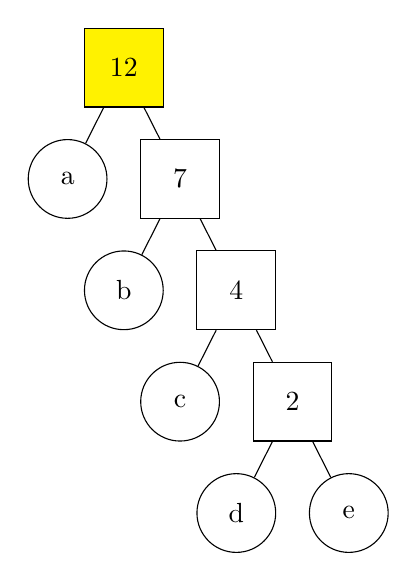
\begin{tikzpicture}[node distance=2cm]

\tikzstyle{ci} = [circle,minimum height=1cm, text centered, draw=black]
\tikzstyle{sq} = [rectangle,minimum height=1cm, minimum width=1cm, text centered, draw=black]
\node (afreq) [sq,fill=yellow] {12};
\node (a) [ci, below left of=afreq, xshift=0.7cm] {a};
\node (bfreq) [sq, below right of=afreq,xshift=-0.7cm] {7};
\node (b) [ci, below left of=bfreq,xshift=0.7cm] {b};
\node (cfreq) [sq, below right of =bfreq,xshift=-0.7cm] {4};
\node (c) [ci, below left of=cfreq,xshift=0.7cm] {c};
\node (edfreq) [sq, below right of=cfreq,xshift=-0.7cm] {2};
\node (d) [ci, below left of=edfreq,xshift=0.7cm] {d};
\node (e) [ci, below right of=edfreq,xshift=-0.7cm] {e}; 
\draw (afreq)--(a);
\draw (bfreq)--(b);
\draw (cfreq)--(c);
\draw (edfreq)--(d);
\draw (edfreq)--(e);
\draw (edfreq)--(cfreq);
\draw (bfreq) -- (cfreq);
\draw (bfreq) -- (afreq);
\end{tikzpicture}
\end{figure}
\noindent To determine the table of codewords, you must refer to the Huffman Tree. The codeword for each left edge is `0', while the right edge is `1'. For example, to get to the letter `$c$', you must go down the edges in this order: right $\rightarrow$ right $\rightarrow$ left. Therefore, the codeword for $c \rightarrowtail 110$. Repeat for all characters and you will get the following codeword table.
\begin{table}[H]
\centering
\begin{tabular}{|c|c|c|c|c|}
\hline
a & b & c & d & e \\ \hline
0 & 10 & 110 & 1110 & 1111 \\ \hline
\end{tabular}
\end{table}
\EOQ
\paragraph{Question 6.} What is the maximal set from the following set of points? Show your steps using a binary tree, that arises from the method of divide-and-conquer.
\begin{equation*}
\{(5,9),(2,3),(9,2),(1,4),(7,3),(4,5),(3,8)\}
\end{equation*}
\hfill {\bf (12 marks)}
\newpage
\paragraph{Answer}\mbox{}\\\\Assume that the left subset will have $\lfloor n/2 \rfloor$ points. Using the first values as a pivot, (4,5) will act as the median when the list has been sorted.
\begin{figure}[H]
\centering
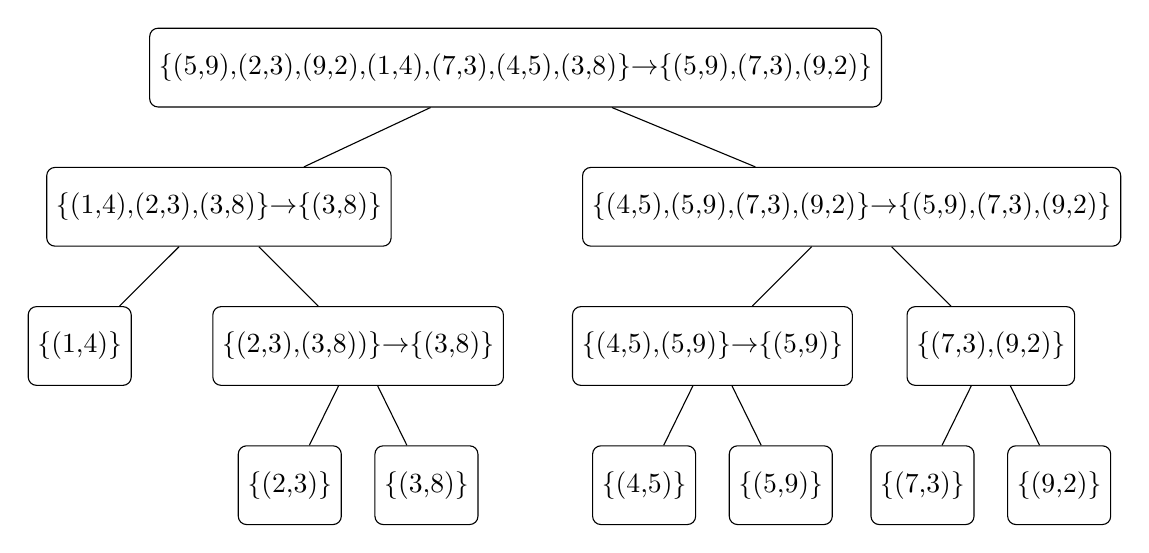
\begin{tikzpicture}[node distance=2.5cm]
\tikzstyle{rr} = [rectangle, rounded corners=3pt, minimum width=1cm, minimum height=1cm, text centered, draw=black]
\node (Top)[rr]{\{(5,9),(2,3),(9,2),(1,4),(7,3),(4,5),(3,8)\}$\rightarrow$\{(5,9),(7,3),(9,2)\}};
\node (L) [rr,below left of=Top, xshift=-2cm]{\{(1,4),(2,3),(3,8)\}$\rightarrow$\{(3,8)\}};
\node (R) [rr,below right of=Top, xshift=2.5cm]{\{(4,5),(5,9),(7,3),(9,2)\}$\rightarrow$\{(5,9),(7,3),(9,2)\}};
\node (LL) [rr,below left of=L] {\{(1,4)\}};
\node (LR) [rr, below right of =L] {\{(2,3),(3,8))\}$\rightarrow$\{(3,8)\}};
\node (LRL) [rr, below left of =LR, xshift=0.9cm] {\{(2,3)\}};
\node (LRR) [rr, below right of =LR,xshift=-0.9cm] {\{(3,8)\}};
\node (RL) [rr, below left of=R] {\{(4,5),(5,9)\}$\rightarrow$\{(5,9)\}};
\node (RR) [rr, below right of=R] {\{(7,3),(9,2)\}};
\node (RLL) [rr, below left of=RL,xshift=0.9cm] {\{(4,5)\}};
\node (RLR) [rr, below right of=RL,xshift=-0.9cm] {\{(5,9)\}};
\node (RRL) [rr, below left of=RR,xshift=0.9cm] {\{(7,3)\}};
\node (RRR) [rr, below right of =RR,xshift=-0.9cm] {\{(9,2)\}};
\draw (Top) -- (L);
\draw (Top) -- (R);
\draw (L) -- (LL);
\draw (L) -- (LR);
\draw (LR) -- (LRL);
\draw (LR) -- (LRR);
\draw (R) -- (RR);
\draw (R) -- (RL);
\draw (RLL) --(RL);
\draw (RLR) --(RL);
\draw (RRL) -- (RR);
\draw (RRR) -- (RR);

\end{tikzpicture}
\end{figure}\mbox{}\\
\noindent
Nodes with one element are not changed (trivial).\\

\noindent
Step \circled{1} \\Sort and identify median\\\\
Step \circled{2} \\Split the values into the left and right subtrees respectively depending on whether the $1^{st}$ values are less than ($<$) or greater than ($>$) the median.\\\\
Step \circled{3} \\Arrays of length 1 are already sorted (trivial).\\\\
Step \circled{4} \\ Combine after you have obtained all leaf nodes, removing all values where $(x_i,y_i)<(x_j,y_j)$ where $i<j$.\\\\Therefore, the maximal set is determined to be the following: \{(5,9),(7,3),(9,2)\}\\\mbox{}\EOQ
\newpage
\paragraph{Question 7.} Let $A,B,C,D$ be matrices with the following dimensions:
\begin{equation*}
A:2\times 2\quad B:2\times 1\quad C:1\times 8\quad D:8\times 8 
\end{equation*}
What is the minimum number of item-wise multiplications required to compute the product $A\ast B\ast C\ast D$? Provide a parenthesization that achieves this minimum.\hfill {\bf (12 marks)}
\paragraph{Answer}\mbox{}\\\\When performing the \textit{Matrix Chain Algorithm}, we must identify the number of matrices that need to undergo multiplication. In this case, we have 4 matrices. As such, we have \{$d_0,\cdots,d_4$\}. $d_i$ represents the dimension of the respective matrix.
\begin{equation*}
\therefore d_0=2\quad d_1=2\quad d_2=1\quad d_3=8\quad d_4=8
\end{equation*} Furthermore, a 4$\times$4 matrix $N$ is created to illustrate the operations that need to be performed.
\begin{figure}[H]
\centering
\begin{tikzpicture}[node distance=0.8cm]
\tikzstyle {sq1}=[rectangle, minimum width=0.8cm, minimum height=0.8cm,draw=black]
\tikzstyle {sqc}=[sq1, fill=yellow!80]
\tikzstyle {txtonly}=[rectangle,minimum width=1cm, minimum height=0.8cm]
\node (00) [sq1] {};
\node (01) [sq1, right of=00] {};
\node (02) [sq1,right of=01] {};
\node (03) [sq1,right of=02] {};
\node (10) [sq1,below of=00] {};
\node (11) [sq1,right of=10] {};
\node (12) [sq1,right of=11] {};
\node (13) [sq1,right of=12] {};
\node (20) [sq1,below of=10] {};
\node (21) [sq1,right of=20] {};
\node (22) [sq1,right of=21] {};
\node (23) [sq1,right of=22] {};
\node (30) [sq1,below of=20] {};
\node (31) [sq1,right of=30] {};
\node (32) [sq1,right of=31] {};
\node (33) [sq1,right of=32] {};
\node (letter) [below left of=10,above left of=20,xshift=-0.5cm, yshift=0.4cm] {$N:$};
\end{tikzpicture}
\end{figure}
\noindent
The order of obtaining the values involves calculation of the \textbf{\underline{diagonals}} first and moving towards the \textbf{\underline{right}}. i.e. Obtaining values for the matrix must strictly follow this order.
\begin{figure}[H]
\centering
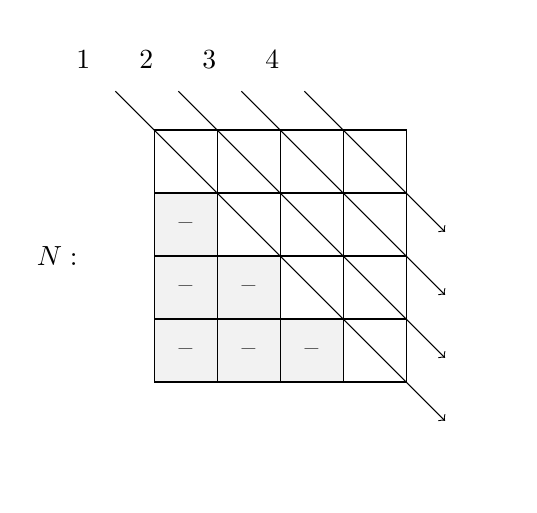
\begin{tikzpicture}[node distance=0.8cm]
\tikzstyle {sq1}=[rectangle, minimum width=0.8cm, minimum height=0.8cm,draw=black]
\tikzstyle {sqc}=[sq1, fill=yellow!80]
\tikzstyle {sqg}=[sq1,fill=gray!10]
\tikzstyle {txtonly}=[rectangle,minimum width=1cm, minimum height=0.8cm]
\tikzstyle{emptynode}=[rectangle,minimum width=0.8cm, minimum height=0.8cm]
\node (00) [sq1] {};
\node (01) [sq1, right of=00] {};
\node (02) [sq1,right of=01] {};
\node (03) [sq1,right of=02] {};
\node (10) [sqg,below of=00] {--};
\node (11) [sq1,right of=10] {};
\node (12) [sq1,right of=11] {};
\node (13) [sq1,right of=12] {};
\node (20) [sqg,below of=10] {--};
\node (21) [sqg,right of=20] {--};
\node (22) [sq1,right of=21] {};
\node (23) [sq1,right of=22] {};
\node (30) [sqg,below of=20] {--};
\node (31) [sqg,right of=30] {--};
\node (32) [sqg,right of=31] {--};
\node (33) [sq1,right of=32] {};
\node (letter) [below left of=10,above left of=20,xshift=-0.5cm, yshift=0.4cm] {$N:$};


\node (fill1) [emptynode,above of=00,xshift=-0.5cm,yshift=0.5cm]{2};
\node (fill0) [emptynode,left of=fill1]{1};
\node (fill2) [emptynode,right of=fill1]{3};
\node (fill3) [emptynode, right of=fill2]{4};

\node (fill4) [emptynode,right of=13,xshift=0.5cm,yshift=-0.5cm]{};
\node (fill5) [emptynode,below of=fill4]{};
\node (fill6) [emptynode,below of=fill5]{};
\node (fill7) [emptynode, below of=fill6]{};
\draw[->] (fill0) -- (fill7);
\draw[->] (fill1) -- (fill6);
\draw[->] (fill2) -- (fill5);
\draw[->] (fill3) -- (fill4);
\end{tikzpicture}
\end{figure}
\noindent The first part of the algorithm requires that the first diagonal be set to 0. i.e. All $N_{i,i}=0 \text{ for } 0\leq i< (\text{Number of matrices})$.\\\\
\begin{minipage}{0.45\textwidth}
\begin{equation*}
\begin{split}
N_{0,0}=0\\
N_{1,1}=0\\
N_{2,2}=0\\
N_{3,3}=0
\end{split}
\end{equation*}
\end{minipage}%
\hfill
\begin{minipage}{0.45\textwidth}\vspace*{0.36cm}
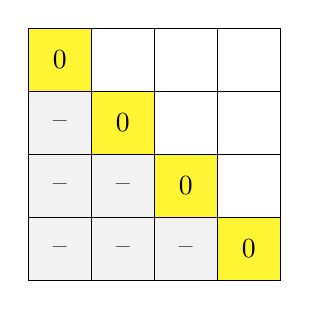
\begin{tikzpicture}[node distance=0.8cm]
\tikzstyle {sq1}=[rectangle, minimum width=0.8cm, minimum height=0.8cm,draw=black]
\tikzstyle {sqc}=[sq1, fill=yellow!80]
\tikzstyle {sqg}=[sq1,fill=gray!10]
\tikzstyle {txtonly}=[rectangle,minimum width=1cm, minimum height=0.8cm]
\tikzstyle{emptynode}=[rectangle,minimum width=0.8cm, minimum height=0.8cm]
\node (00) [sqc] {0};
\node (01) [sq1, right of=00] {};
\node (02) [sq1,right of=01] {};
\node (03) [sq1,right of=02] {};
\node (10) [sqg,below of=00] {--};
\node (11) [sqc,right of=10] {0};
\node (12) [sq1,right of=11] {};
\node (13) [sq1,right of=12] {};
\node (20) [sqg,below of=10] {--};
\node (21) [sqg,right of=20] {--};
\node (22) [sqc,right of=21] {0};
\node (23) [sq1,right of=22] {};
\node (30) [sqg,below of=20] {--};
\node (31) [sqg,right of=30] {--};
\node (32) [sqg,right of=31] {--};
\node (33) [sqc,right of=32] {0};
\end{tikzpicture}

\end{minipage}
\\\\\\
Calculating all other matrix index values requires the use of the formula:
\begin{equation*}
N_{i,j}=\min_{i\leq k<j} \{N_{i,k}+N_{k+1,j}+d_i d_{k+1} d_{j+1}\}
\end{equation*}
Following the numbered diagonals, the remaining indexes are worked out in order.\\\\(Second diagonal)
\begin{equation*}
\begin{split}
N_{0,1}\Rightarrow i=0, j=1 \Rightarrow k=0 &\Rightarrow \min_{0\leq k<1}\{N_{0,0}+N_{1,1}+d_0d_1d_2\}\\
&=\min_{0\leq k<1}\{0+0+4\}\\
&=4\\
N_{1,2}\Rightarrow i=1, j=2 \Rightarrow k=1 &\Rightarrow \min_{1\leq k<2}\{N_{1,1}+N_{2,2}+d_1d_2d_3\}\\
&=\min_{1\leq k<2}\{0+0+16\}\\
&=16\\
N_{2,3}\Rightarrow i=2, j=3 \Rightarrow k=2 &\Rightarrow \min_{2\leq k<3}\{N_{2,2}+N_{3,3}+d_2d_3d_4\}\\
&=\min_{2\leq k<3}\{0+0+64\}\\
&=64\\
\end{split}
\end{equation*}
\begin{figure}[H]
\centering
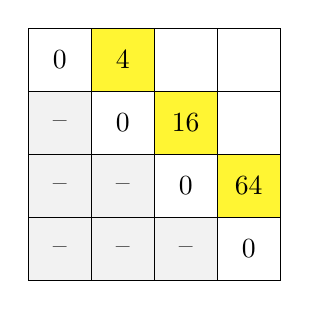
\begin{tikzpicture}[node distance=0.8cm]
\tikzstyle {sq1}=[rectangle, minimum width=0.8cm, minimum height=0.8cm,draw=black]
\tikzstyle {sqc}=[sq1, fill=yellow!80]
\tikzstyle {sqg}=[sq1,fill=gray!10]
\tikzstyle {txtonly}=[rectangle,minimum width=1cm, minimum height=0.8cm]
\tikzstyle{emptynode}=[rectangle,minimum width=0.8cm, minimum height=0.8cm]
\node (00) [sq1] {0};
\node (01) [sqc, right of=00] {4};
\node (02) [sq1,right of=01] {};
\node (03) [sq1,right of=02] {};
\node (10) [sqg,below of=00] {--};
\node (11) [sq1,right of=10] {0};
\node (12) [sqc,right of=11] {16};
\node (13) [sq1,right of=12] {};
\node (20) [sqg,below of=10] {--};
\node (21) [sqg,right of=20] {--};
\node (22) [sq1,right of=21] {0};
\node (23) [sqc,right of=22] {64};
\node (30) [sqg,below of=20] {--};
\node (31) [sqg,right of=30] {--};
\node (32) [sqg,right of=31] {--};
\node (33) [sq1,right of=32] {0};
\end{tikzpicture}
\end{figure}
\noindent (Third diagonal)
\begin{equation*}
\begin{split}
N_{0,2}\Rightarrow i=0, j=2 \Rightarrow k=\{0,1\} &\Rightarrow \min_{0\leq k<2}\{N_{0,0}+N_{1,2}+d_0d_1d_3,N_{0,1}+N_{2,2}+d_0d_2d_3\}\\
&=\min_{0\leq k<2}\{0+16+32,4+0+16\}\\
&=20\\
N_{1,3}\Rightarrow i=1, j=2 \Rightarrow k=\{1,2\} &\Rightarrow \min_{1\leq k<3}\{N_{1,1}+N_{2,3}+d_1d_2d_4,N_{1,2}+N_{3,3}+d_1d_3d_4\}\\
&=\min_{1\leq k<3}\{0+64+16,16+0+128\}\\
&=80\\
\end{split}
\end{equation*}
\begin{figure}[H]
\centering
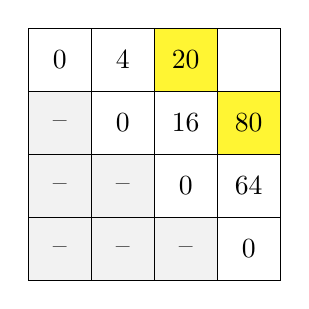
\begin{tikzpicture}[node distance=0.8cm]
\tikzstyle {sq1}=[rectangle, minimum width=0.8cm, minimum height=0.8cm,draw=black]
\tikzstyle {sqc}=[sq1, fill=yellow!80]
\tikzstyle {sqg}=[sq1,fill=gray!10]
\tikzstyle {txtonly}=[rectangle,minimum width=1cm, minimum height=0.8cm]
\tikzstyle{emptynode}=[rectangle,minimum width=0.8cm, minimum height=0.8cm]
\node (00) [sq1] {0};
\node (01) [sq1, right of=00] {4};
\node (02) [sqc,right of=01] {20};
\node (03) [sq1,right of=02] {};
\node (10) [sqg,below of=00] {--};
\node (11) [sq1,right of=10] {0};
\node (12) [sq1,right of=11] {16};
\node (13) [sqc,right of=12] {80};
\node (20) [sqg,below of=10] {--};
\node (21) [sqg,right of=20] {--};
\node (22) [sq1,right of=21] {0};
\node (23) [sq1,right of=22] {64};
\node (30) [sqg,below of=20] {--};
\node (31) [sqg,right of=30] {--};
\node (32) [sqg,right of=31] {--};
\node (33) [sq1,right of=32] {0};
\end{tikzpicture}
\end{figure}
\noindent (Last diagonal)
\begin{equation*}
\begin{split}
N_{0,3}&\Rightarrow i=0, j=3 \Rightarrow k=\{0,1,2\} \\&\Rightarrow \min_{0\leq k<3}\{N_{0,0}+N_{1,3}+d_0d_1d_4,N_{0,1}+N_{2,3}+d_0d_2d_4,N_{0,2}+N_{3,3}+d_0d_3d_4\}\\
&=\min_{0\leq k<3}\{0+80+32,4+64+16,20+0+128\}\\
&=84
\end{split}
\end{equation*}
\begin{figure}[H]
\centering
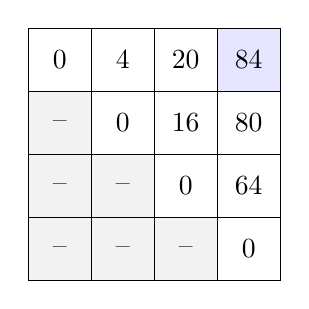
\begin{tikzpicture}[node distance=0.8cm]
\tikzstyle {sq1}=[rectangle, minimum width=0.8cm, minimum height=0.8cm,draw=black]
\tikzstyle {sqc}=[sq1, fill=yellow!80]
\tikzstyle {sqg}=[sq1,fill=gray!10]
\tikzstyle {txtonly}=[rectangle,minimum width=1cm, minimum height=0.8cm]
\tikzstyle{emptynode}=[rectangle,minimum width=0.8cm, minimum height=0.8cm]
\node (00) [sq1] {0};
\node (01) [sq1, right of=00] {4};
\node (02) [sq1,right of=01] {20};
\node (03) [sq1,right of=02,fill=blue!10] {84};
\node (10) [sqg,below of=00] {--};
\node (11) [sq1,right of=10] {0};
\node (12) [sq1,right of=11] {16};
\node (13) [sq1,right of=12] {80};
\node (20) [sqg,below of=10] {--};
\node (21) [sqg,right of=20] {--};
\node (22) [sq1,right of=21] {0};
\node (23) [sq1,right of=22] {64};
\node (30) [sqg,below of=20] {--};
\node (31) [sqg,right of=30] {--};
\node (32) [sqg,right of=31] {--};
\node (33) [sq1,right of=32] {0};
\end{tikzpicture}
\end{figure}
\noindent From $N_{0,3}$, we are able to tell that the minimum number of item-wise multiplications required is 84.\\\\To determine the parenthesization for the least number of item-wise multiplications, we need to work backwards.
$N_{0,3}$ is obtained from $N_{0,1}+N_{2,3}+d_0d_2d_4$, implying that matrices 0 to 1 are enclosed within a single bracket. i.e. $(A\ast B)\ast C \ast D$. No further analysis of paranthesization of $C$ and $D$ are required since there are only two matrices. Similarly, we also see that matrices 2 to 3 are enclosed within a single bracket. i.e. $(A\ast B)\ast (C \ast D)$.\\\\Note that when looking at the term $N_{i,j}$, it means that matrices $i$ to $j$ inclusive are enclosed within 1 bracket and should be checked to determine whether further paranthesization is required.\\\\
The answer for this question is 84 item-wise multiplications required and the respective paranthesization that gives the solution is this: $(A\ast B)\ast (C \ast D)$\\\mbox{}\EOQ
\bigskip
\vfill
\begin{center}{\bf END OF PAPER}\end{center}
\end{document}
